\section{Propuesta}
\label{sec:propuesta}



\subsection{Diseños propuestos}
\label{sec:disenos}

La propuesta consiste en desarrollar una red dinámica eficiente que
sea robusta ante posibles fallas en la interconexión física de los
datacenters. Para esto se ha contactado a varios proveedores de
dispositivos ópticos \emph{DWDM} para cotizar los distintos equipos
que necesitan ser instalados en los nodos de la red y así poder contar
con un valor estimado de el costo de capital del proyecto.

Los proveedores de redes contactados fueron:
\begin{itemize}
\item Alcatel
\item Ericsson
\item Huawei
\item Nokia NSN
\item Siemens
\item Sonda (representantes de Cisco en Chile)
\end{itemize}

A la par de esta cotización, se ha desarrollado un modelo
probabilístico para la programación de los dispositivos \emph{ROADM}
que asegura un valor de mínimo de disponibilidad de la red; esto
determina principalmente el \emph{SLA} estimado de la red (mayores
detalles se exponen en la sección \ref{sec:SLA}).

Este modelo probabilístico se programará en el controlador
\emph{ROADM} de la red, haciendo que el requerimiento en \emph{SLA} de
la red sea en efecto una variable de entrada para el diseño.

\begin{figure}[h]
\centering
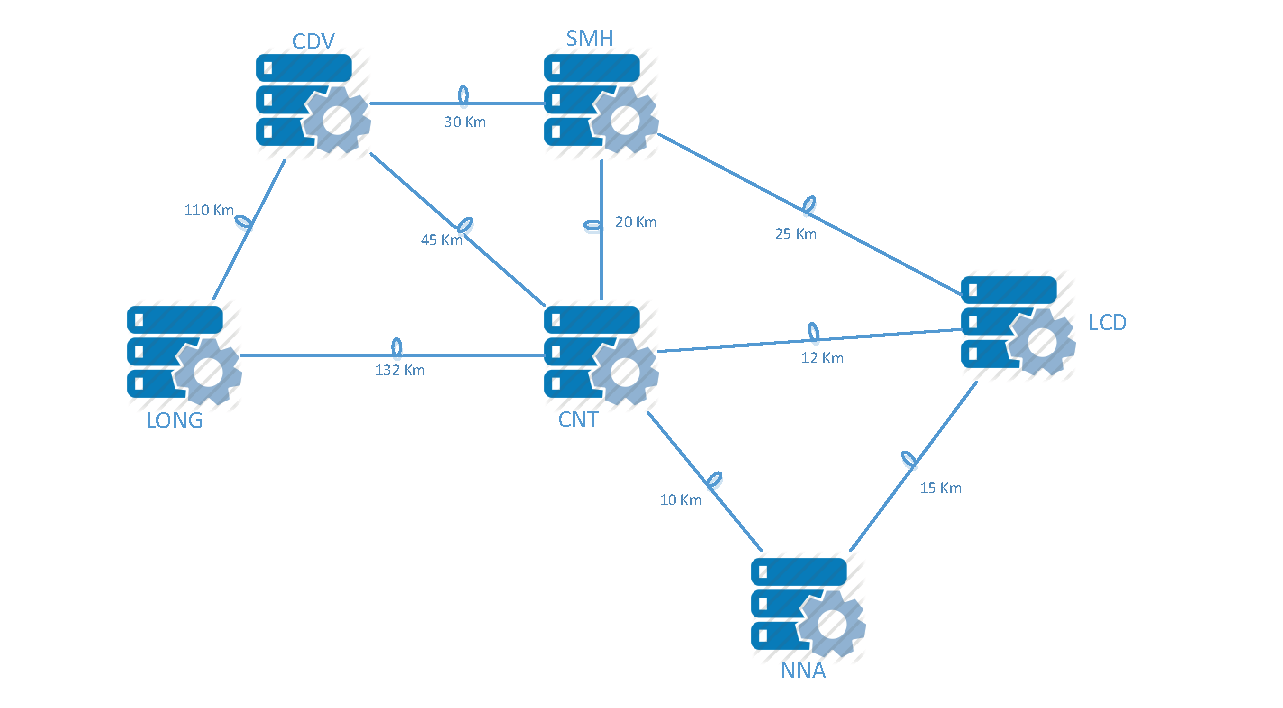
\includegraphics[width=0.7\textwidth]{Imagenes/Diagrama_Fibra_Oscura.eps}
\caption{Diagrama inicial de red oscura preexistente. Este diagrama se
  presenta a los distintos proveedores para que se pueda estimar el
  número de amplificadores, compensadores de dispersión necesarios,
  etcétera.}
\end{figure}

% Para la definición de la red, fue necesario definir las rutas que
% conectan cada par de \textit{DataCenters}.  Para obtener un modelo
% robusto a cortes, es necesario que exista más de una ruta entre cada
% par de puntos o almenos cierta cantidad que garantize los
% requerimientos predefinidos.

% La forma en que se diseño esta red, utiliza ciertas características
% intrínsicas de la red de fibra oscura actual. Por ejemplo se ciñe a
% las tasas anuales de corte para la fibra utilizada (AEG-10
% \textbf{CORREGIR}), y también a las capacidades requeridas por cada
% protocolo GE y (balblalbal)


% El conjunto de rutas alternativas debe cumplir un criterio de umbral
% de seguridad, si no lo cumple se agregarán más rutas alternativas
% hasta que se logre dicho objetivo.

Hasta el momento, no ha habido respuesta de los proveedores.

\subsection{Propuesta final}
\label{sec:ppfinal}

